%%%%%%%%%%%%%%%%%%%%%%%%%%%%%%%%%%%%%%%%%
% Short Three-Column Newsletter
% LaTeX Template
% Version 1.0 (11/9/13)
%
% Original author:
% Frits Wenneker (http://www.howtotex.com) 
% With extensive modifications by:
% Vel (vel@latextemplates.com)
% 
% This template has been downloaded from:
% http://www.LaTeXTemplates.com
%
% License:
% CC BY-NC-SA 3.0 (http://creativecommons.org/licenses/by-nc-sa/3.0/)
%
%%%%%%%%%%%%%%%%%%%%%%%%%%%%%%%%%%%%%%%%%

%----------------------------------------------------------------------------------------
%	PACKAGES AND DOCUMENT CONFIGURATIONS
%----------------------------------------------------------------------------------------

\documentclass[10pt,a4paper,ngerman,twoside]{article} % Paper type (a4paper, usletter or legal) and font size (10, 11 or 12)

%\setlength\topmargin{-80mm} % Top margin
\setlength\topmargin{-48pt} % Top margin
\setlength\headheight{0pt} % Header height
\setlength\textwidth{7.0in} % Text width
\setlength\textheight{9.5in} % Text height
\setlength\oddsidemargin{-30pt} % Left margin
\setlength\evensidemargin{-30pt} % Left margin (even pages) - only relevant with 'twoside' article option
%\setlength\inner{4cm}
%\setlenfth\outer{2cm}
%\usepackage{geometry}
%\geometry{bindingoffset=20mm}
%\setlength\bindingoffset{2cm}

\usepackage{charter} % Charter font for main content

\frenchspacing % Reduces space after periods to make text more compact for a three-column layout
\usepackage{babel}
\usepackage[utf8]{inputenc}
\usepackage{graphicx} % Required for including images
\usepackage{amssymb} % Math packages
\usepackage{amsmath} 
\usepackage{multicol} % Required for the three-column layout of the document
\usepackage{url} % Clickable links
\usepackage{enumitem} % Reduces the amount of space within and between lists with [noitemsep,nolistsep]
\usepackage{marvosym} % Required for the use of symbols
\usepackage{wrapfig} % Allows wrapping text around figures
%\usepackage[T1]{fontenc} % Use 8-bit encoding that has 256 glyphs
\usepackage{datetime} % Required for defining a custom date style
\newdateformat{mydate}{\monthname[\THEMONTH] \THEYEAR} % Set a custom date format
\usepackage[pdfpagemode=FullScreen, colorlinks=false]{hyperref} % Link colors and PDF behavior in Acrobat
\usepackage{fancyhdr} % Required to define custom headers/footers
\usepackage{hyperref} % funktioniert nicht ?
\pagestyle{fancy} % Enables the custom headers/footers for all pages following this

%-----------------------------------------------------------
% Header and footer
\lfoot{\footnotesize % Left footer containing newsletter contact information
%\begin{wrapfigure}{l}{2.0cm}
%
\includegraphics[width=2cm]{ccbysa88x31.png} 
%\end{wrapfigure}
R.I.S. Journal Ausgabe 001, Jänner 2014: \textbf{R}emix, \textbf{I}mprove, \textbf{S}hare. Das freie, creativ-commons lizensierte Journal.  \\
\Mundus\ Download und andere Formate: \href{http://spielend-programmieren.at/de:ris:start}{\texttt{spielend-programmieren.at/de:ris:start}} \quad
%\Telefon\ (000) 111-1111 \quad
\Letter\ \href{mailto:horst.jens@spielend-programmieren.at}{horst.jens@spielend-programmieren.at}
}

\cfoot{} % Empty center footer

\rfoot{\footnotesize ~\\ Seite \thepage} % Right footer - page counter

\renewcommand{\headrulewidth}{0.0pt} % No horizontal rule for the header
\renewcommand{\footrulewidth}{0.4pt} % Horizontal rule separating the footer from the document
%-----------------------------------------------------------

%-----------------------------------------------------------
% Define separators
\newcommand{\HorRule}[1]{\noindent\rule{\linewidth}{#1}} % Creates a horizontal rule
\newcommand{\SepRule}{\noindent	% Creates a shorter separator rule
\begin{center}
\rule{250pt}{1pt} % Page width and rule width
\end{center}
}
\newcommand{\Trenner}{\noindent
\begin{center}
\rule{100pt}{1pt}
\end{center}
}
%-----------------------------------------------------------

%-----------------------------------------------------------
% Define title and article styles
\newcommand{\NewsletterName}[1]{ % Newsletter title
\begin{center}
\Huge \usefont{T1}{fvs}{b}{n} % Use the Bera Sans Bold font
#1
\end{center}	
\par \normalsize \normalfont}

\newcommand{\JournalIssue}[1]{ % Date and issue number at the top of the newsletter
%\hfill \textsc{\mydate \today, No #1} % Right-aligned date and issue number
\hfill \textsc{Jänner 2014, Ausgabe 001}
\par \normalsize \normalfont}

\newcommand{\NewsItem}[1]{ % News item title
\usefont{T1}{fvs}{n}{n} % Use the Bera Sans Normal font
\vspace{24pt}\large #1\vspace{3pt} % Print the title with space around it in a larger font size
\par \normalsize \normalfont}

\newcommand{\NewsAuthor}[1]{ % Author name under the item title
\hfill von \textsc{#1} \vspace{20pt} % Right-aligned author name in small caps with space after it
\par \normalfont}		

%----------------------------------------------------------------------------------------
%	TITLE
%----------------------------------------------------------------------------------------

\begin{document}

\JournalIssue{1} % Issue number
\NewsletterName{R.I.S. Journal} % Newsletter title
%\begin{center}
%\textbf{R}emix \textbf{I}mprove \textbf{S}hare - das freie Journal für Open Source Education
%\end{center}
\noindent\HorRule{3pt} \\[-0.75\baselineskip] % Thick horizontal rule
\HorRule{1pt} % Thin horizontal rule



%\setlength{\columnsep}{16pt} % Uncomment to manually change the white space between columns
%\begin{multicols}{3} % Begin the three-column layout

%----------------------------------------------------------------------------------------
%	OTHER NEWS
%----------------------------------------------------------------------------------------
%-----------------------------------------------------------
%
%-----------------------------------------------------------
%RIS-Journal Titel (Titelgrafik hier einfügen)
\begin{multicols}{3}
\NewsItem{}
\section*{Fdroid Installationsanleitung}
\label{fdroid}
\NewsAuthor{Horst JENS}

\textbf{In diesem Tutorial wird erklärt wie Sie sich auf einem Android Smartphone oder Tablet das Fdroid Repository für freie (free/libre Open Source) Software installieren, um eine sinnvolle Ergänzung zum Google Play Store zu haben.}

%\begin{center}
%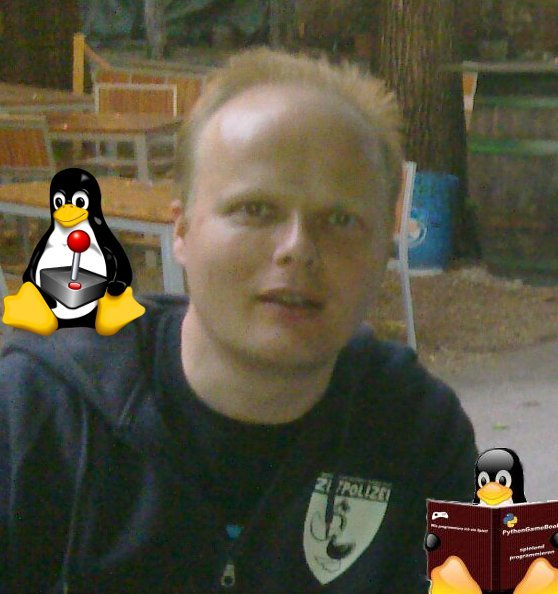
\includegraphics[width=\linewidth]{fdroid/horst2011mitdoppeltux.jpg} \\
%\footnotesize{Horst JENS. Bildrechte: [9], cc-by-sa}
%\end{center}
\begin{center}
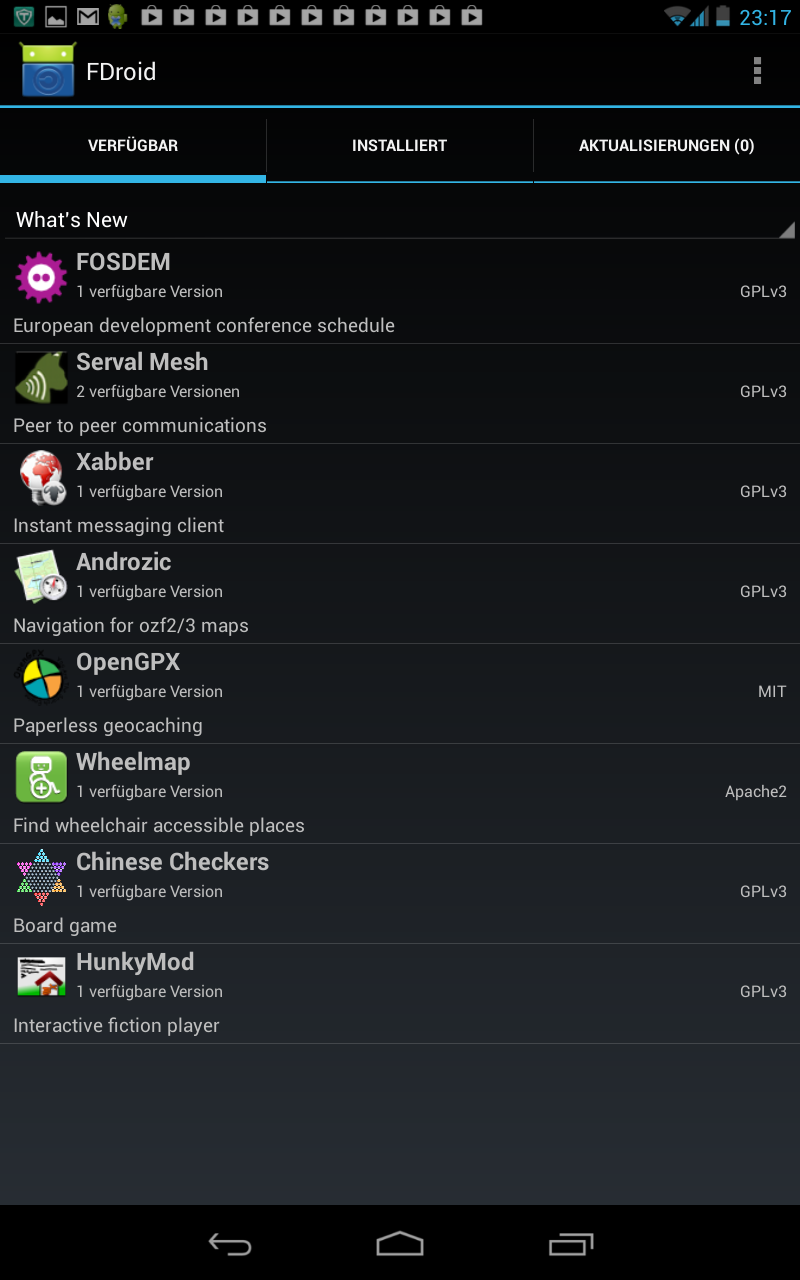
\includegraphics[width=\linewidth]{fdroid/fdroid2.png} \\
\footnotesize{Fdroid}
\end{center}
\subsection*{Das freies Softwarerepository Fdroid für Android installieren}

Wirklich \href{http://de.wikipedia.org/wiki/Freie_Software}{\textit{freie (free/libre Open Source) Software [1]}} für \href{http://www.android.com/}{\textit{Android [2]}}-Geräte zu finden ist gar nicht so leicht: Der \href{https://play.google.com/store}{\textit{Google Play Store [3]}} lässt sich zwar nach "kostenlos" durchsuchen, aber kostenlos ( "free as beer" ) ist eben nicht das selbe wie wirklich frei (quelloffen, "free as freedom") im Sinne der \href{http://de.wikipedia.org/wiki/GNU_General_Public_License}{\textit{GPL Lizenz [4]}}. Mit relativ wenig Aufwand ist es allerdings möglich, auf Android-Geräten ("Devices" wie Smartphones, Tablets, ...) ein alternatives Softwareverzeichnis, ein sogenanntes \href{http://de.wikipedia.org/wiki/Repository}{\textit{Repository [5]}} zu installieren, welches nur wirklich freie Software anbietet. Keine \href{http://de.wikipedia.org/wiki/Crippleware}{\textit{Crippleware [6]}}, keine nervenden Werbebanner, kein geheimer Programmcode. Dieses Tutorial erklärt wie es geht:


\subsection*{Anleitung:}
Die folgende Schritte möglichst direkt mit dem Android-Gerät ausführen:

\textbf{Gerätezugriff gewähren}: Die FDroid-App verlang beim Installieren weitgehende Rechte auf dem Android-Gerät, um weitere Apps installieren und löschen zu dürfen:

\begin{itemize}
\item Im Systemmenü des Android-Geräts unter \emph{Einstellungen - Sicherheit} die Option \emph{Unbekannte Herkunft - Installation von Apps aus anderen Quellen als dem PlayStore zulassen} anklicken (das Häckchen muss gesetzt sein).
\item Die Website \url{http://f-droid.org/} ansurfen und die Seite durchlesen. Die Seite akzeptiert Spenden per Flattr, PayPal und Bitcoin. Im Fdroid FAQ (im Wiki) wird u.a. erklärt, warum FDroid NICHT im Google Play Store drin ist (Konkurrenzverbot).
\item Direkt auf der FDroid-Website kann man mit dem Menüpunkt \emph{Browse} schauen was für freie Apps es gibt, um zu entscheiden ob man FDroid überhaupt braucht.
\item Direkt auf der \href{http://f-droid.org/}{\textit{FDroid-Website [7]}} ist ein Download-Link mit dem man die Datei \href{http://f-droid.org/FDroid.apk}{\textit{FDroid.apk [8]}} downloaden kann. Oder man scannt mit dem Android-Device diesen QR-Code:

\begin{center}

\includegraphics[width=4cm]{fdroid/fdroidurl.png}
\end{center}

\item Die heruntergeladene Datei \emph{FDroid.apk} öffnen. Dazu oben in der Statusleiste auf das Downloadsymbol (Pfeil nach unten) mit dem Finger "wischen" und auf die Meldung \emph{Download abgeschlossen} drauf klicken. Nach einigem Nachfragen wird die FDroid-App auf dem Android-Device installiert.
\item Die FDroid-App im App-Menü des Android-Geräts suchen und starten.
\item Wenn die FDroid-App läuft, den Menü-Button drücken und \emph{Update} wählen. Nach einiger Zeit erscheint eine Liste verfügbarer freier Apps, die man mittels "Install", "Update" und "Remove" managen kann.
\item Um zu schauen ob es neuere Versionen von freien Apps gibt muss man FDRoid starten und im Menü auf update klicken. Die Apps werden NICHT über den Google Play Store aktualisiert.
\item Es empfiehlt sich manchmal, nicht die allerneuste Version einer App zu installieren sondern die "vorletzte" Version (die 2. von obenin der Versionliste). Dadurch verzichtet man zwar auf die allerneusten Features, erspart sich dafür die allerneusten Fehler.
\item FDroid selbst lässt sich mittels FDroid updaten :-)
\end{itemize}

\subsection*{Fachbegriffe:}

~~~\href{http://de.wikipedia.org/wiki/Freie_Software}{\textbf{freie Software [1]}}: ist nicht zu verwechseln mit kostenloser Software (Freeware). Freie Software gewährt die \textbf{4 Grundfreiheiten} gemäß der \textbf{GPL-Lizenz} und ermöglicht es, den Quellcode (SourceCode) der Software anzuschauen, zu benutzen, zu verändern und zu kopieren und weiterzugeben.

\href{http://de.wikipedia.org/wiki/GNU_General_Public_License}{Gnu Public License (GPL)} [4]
\begin{center}

\includegraphics[width=4cm]{fdroid/fdroid_gpl_logo.png}
\end{center}
garantiert dem Nutzer der Software die 4 Grundfreiheiten \textbf{use, study, share, improve}. Näheres dazu können Sie im Leitartikel dieser Ausgabe nachlesen. \\

\href{http://www.android.com/}{\textbf{Android}} [2]: Ein freies, Linux-basiertes Betriebssystem, vor allem für Smartphones und Tablets. Android selbst ist GPL-lizensierte, freie Software, aber viele der Apps die auf Android laufen (z.B. Skype, aber auch der \textbf{Google Play Store} sind unfreie Software.. \\

\href{http://de.wikipedia.org/wiki/Google_Play}{\textbf{Google Play Store}} ist ein von Google vorinstallierter Softwareshop für Android-Geräte, ähnlich Apple's \href{http://de.wikipedia.org/wiki/AppStore}{AppStore}. Derzeit (Dez 2013) lässt sich Google's Play Store zwar nach kostenlosen Apps filtern, nicht aber nach freien Lizenzen. \\

\href{http://de.wikipedia.org/wiki/Repository}{\textbf{Software-Repository}} [5]: Ein Verzeichnis installierbarer Software (oder Apps) welches eine Versionsverwaltung beinhaltet und das installieren, löschen, updaten und verwalten von Software oder Apps erlaubt. Im Linux-Bereich hat fast jede Distribution ein eigenes Repository (z.B. Debian, Ubuntu, Suse...). Man kann sich auch selbst Repositorys erstellen. \\

\href{http://de.wikipedia.org/wiki/Crippleware}{\textbf{Crippleware, Krüppelware}}: ein verächtlicher Begriff für kostenlose Versionen von Software, deren Leistungsumfang stark eingeschränkt ist und erst nach einer entsprechenden Zahlung sinnvoll verwendbar ist. Viele Apps im Google Play Store sind in der "kostenlos" Variante als Crippleware zu bezeichnen, da ihnen entweder wichtige Features fehlen oder weil sie den Nutzer ständig durch Werbebanner nerven, bis er ein kostenpflichtiges Upgrade zur Vollversion durchführt.

\textbf{Danksagung:} \\
Die Android-Screenshots wurden von Phillip Seibt erstellt.

\subsection*{Download, Feedback:}
\footnotesize{
Download: Ordner \texttt{fdroid} \Mundus\ \href{http://spielend-programmieren.at/risjournal/001}{spielend-programmieren.at/risjournal/001}\\
Startseite:\\
\href{http://spielend-programmieren.at/de:ris:001}{spielend-programmieren.at/de:ris:001}\\ 
\Letter\:  horst.jens@spielend-programmieren.at \\}
\normalsize{}

\subsection*{Lizenz, Quellen:}
\begin{wrapfigure}{l}{2.0cm}

\includegraphics[width=2cm]{fdroid/ccbysa88x31.png}
\end{wrapfigure}
Dieses Material steht unter der Creative-Commons-Lizenz Namensnennung - Weitergabe unter gleichen Bedingungen 4.0 International. Um eine Kopie dieser Lizenz zu sehen, besuchen Sie \url{http://creativecommons.org/licenses/by-sa/4.0/deed.de}. \\

\textbf{Quellen:} \\
{[}1{]} \href{http://de.wikipedia.org/wiki/Freie_Software}{wikipedia/Freie-Software} \\
{[}2{]} \href{http://www.android.com}{android.com} \\
{[}3{]} \href{https://play.google.com/store}{play.google.com} \\
{[}4{]} \href{http://de.wikipedia.org/wiki/GNU_General_Public_License}{http://goo.gl/4UTW5B} \\
{[}5{]} \href{http://de.wikipedia.org/wiki/Repository}{de.wikipedia.org/wiki/Repository} \\
{[}6{]} \href{http://de.wikipedia.org/wiki/Crippleware}{de.wikipedia.org/wiki/Crippleware} \\
{[}7{]} \href{http://f-droid.org/}{f-droid.org} \\
{[}8{]} \href{http://f-droid.org/FDroid.apk}{f-droid.org/FDroid.apk} \\
{[}9{]} \href{http://spielend-programmieren.at}{spielend-programmieren} 
\end{multicols}
\SepRule
%-----------------------------------------------------------
\end{document}
